%% entwurf.tex
%% $Id: entwurf.tex 61 2012-05-03 13:58:03Z bless $
%%

\chapter{Conceptual Design and Implementation}
\label{ch:Conceptual Design}
%% ==============================
\par{
Without further ado, design and implementation of the initial ideas began. As Section \ref{ch:Analysis} showed, there are some potentially promising improvements to be made to run length encoding, but how well they scale and work on a larger input with versatile symbols or bytes has to be determined.
}
%% ==============================
\section{Preprocessing}
%% ==============================
\label{ch:Conceptual Design:sec:Preprocessing}

%% ==============================
\subsection{Vertical Byte Reading}
%% ==============================
\label{ch:Conceptual Design:sec:Parallel Byte Reading}
\par{
Implementing the vertical reading of the input shown in Section \ref{ch:Analysis:sec:Improvements by Preprocessing:subSec:vertReading} was not hard but it should be kept in mind that the size of the input chunks has to be divisible by the size of 8. Otherwise parsing it into an Array of Bytes results in the last Byte having some padding which might cause problems later on.  By collecting the bits into a proprietary data structure, we avoid this problem but working with bytes internally should be easier. For larger files it should also be possible to work in space and writing the output on the fly during the reading process. Nonetheless both ways of collecting all bits of identical significance and writing on the fly are implemented.}

\subsubsection{First Ideas}
\par{
Initially some other ideas have been followed with very poor results. One idea was arranging all input bits in a Matrix or square Matrix in a way it would still be receivable later on. This way other methods from linear algebra would have been applicable to the input data, so that the construction of a triangular matrix or other preprocessing would result in long runs of zeros. Difficulties in the construction and transformation of the Data lead to the abandonment of this approach and the already described vertical interpretation was used further on.}

\subsubsection{Other Difficulties}
\par{
Other difficulties arose while performing bit operations, because it became slow on larger workloads. This and other issues where solved by using the Kotlin library  \href{https://discuss.kotlinlang.org/t/i-o-streams-for-kotlin/9802}{IOStreams for Kotlin}} which also allows most operations to be performed on the stream instead of reading all data to encode and then working in memory.

\subsubsection{Compression improvements trough vertical reading}
\par{
First results of just plain binary RLE on the vertical interpretation improved its overall performance and achieved a small edge over regular binary RLE with a slightly smaller expansion but it is still not as good as byte wise RLE with a small run value of 2 bits.
\begin{table}[H]
	\centering
	\begin{tabular}{r|r|r}	
		bits per rle number & ratio in \% & bits per symbol in $\frac{bits}{symbol}$\\
		\hline
		8 & 255.22 & 20.41\\
		7 & 224.45 & 17.95\\
		6 & 194.74 & 15.57\\
		5 & 167.04 & 13.36\\
		4 & 142.58 & 11.40\\
		3 & 127.80 & 10.22\\
		2 & 139.79 & 11.18 \\
	\end{tabular}
	\caption{Binary RLE on vertical interpreted data}
	\label{tab:t30 binary RLE on vertical interpreted data}
\end{table}
}

\par{
If we take a closer look on each file, we see similar results compared to the original proposed binary RLE, where most files had a compression ratio of above 1 with 3 bits per RLE encoded number, except for the file \textit{pic}. Average sizes are increasing again with more bits per run up to 2.5 times its original size and also the file \textit{pic} has the best compression ratio. This time although it is at its peak using 6 bits per RLE run and only achieves a compression of 3.67 $\frac{bits}{symbol}$ compared to 1.56 $\frac{bits}{symbol}$ with simple binary RLE. These results were quite far from the desired outcome which mainly arose because increasing the bits per run improved the result for the most significant bits but also degraded the results for the other bits. So the idea of encoding the bits of different significance with different RLE schemes with varying bits per run arose, to solve this issue.  
}

\subsection{Varying maximum run lengths}
\label{ch:Conceptual Design:sec:var lengths}
\par{
This time the most significant bits have been encoded with more bits per run than the other ones and after bench marking every combination, it turned out, with 2 bits per run and 5 bits per run for the 3 most significant bits, it improved by another 4 percent with most files having a $\frac{bits}{symbol}$ ratio of only slightly above 9. More specifically some textual files are close to 8, which relates to the earlier mentioned ASCII fragments in UTF-8 encoding. This time higher possible runs on this position resulted in fewer runs in total, so in a better compression overall. Applying this increase to more than the most significant bit lead to a decrease in performance, which most likely related to the shorter runs on lower order bits, seen in Section \ref{ch:Analysis:sec:Improvements by Preprocessing:subSec:vertReading}. Therefore this idea was applied again but with a much finer granularity and every combination of different run lengths of every bit could be tried out. For reference, this mapping can be described by a vector $v_i$ with 8 components $v_1,v_2,...,v_8$ each with values greater 1. Each component corresponds to the bits per run stored for the bit number $i$ of each byte.
}
\par{
Testing out every reasonable combination of different run lengths would imply running $8^8$ combinations because every of the 8 bits could be encoded with 2 to 10 bits per run. Assuming around 10 seconds for each encoding round would still result in somewhat around 46 thousand hours of computing which is clearly to much. Even using multi-threading would not resolve this issue so the computation had to be further reduced. By trying only a few specific combinations we assume to be good, we can then selectively small changes to improve further. This way the results were improved and the compression result was lowered around 7 percent points to $112.41\%$ of its original size instead of 127\% with a fix length for every bits position as shown in figure \ref{tab:t50:Calgary Corpus encoded, vertical encoding, using bits per run: (2, 2, 2, 2, 3, 4, 3, 7)}, but this was still far from the desired state. Most files still increased in size except the file \textit{pic}, even though all bits could be encoded differently but the average run length of the lower bits must be very low if 2 bits per RLE number achieved best results. To increase the average run length overall, the already described byte mapping was applied to the input data.
}
\begin{table}[h]
	\centering
	\begin{tabular}{r|r|r|r|r}	
		file & size original & size encoded & ratio in \% & $\frac{bits}{symbol}$\\
		\hline
bib & 111261 & 129424 & 116.32 & 9.31 \\
book1 & 768771 & 820463 & 106.72 & 8.54 \\
book2 & 610856 & 659811 & 108.01 & 8.64 \\
geo & 102400 & 162274 & 158.47 & 12.68 \\
news & 377109 & 400810 & 106.28 & 8.50 \\
obj1 & 21504 & 31592 & 146.91 & 11.75 \\
obj2 & 246814 & 379591 & 153.80 & 12.30 \\
paper1 & 53161 & 57654 & 108.45 & 8.68 \\
paper2 & 82199 & 88121 & 107.20 & 8.58 \\
pic & 513216 & 533254 & 103.90 & 8.31 \\
progc & 39611 & 41360 & 104.42 & 8.35 \\
progl & 71646 & 74554 & 104.06 & 8.32 \\
progp & 49379 & 53403 & 108.15 & 8.65 \\
trans & 93695 & 99818 & 106.54 & 8.52 \\
		\hline
		all files & 3145718 & 3536225 & 112.41 & 8.99
	\end{tabular}
	\caption{Calgary Corpus encoded, vertical encoding, using bits per run: (2, 2, 2, 2, 3, 4, 3, 7)}
	\label{tab:t50:Calgary Corpus encoded, vertical encoding, using bits per run: (2, 2, 2, 2, 3, 4, 3, 7)}
\end{table}

\subsection{Byte remapping}
\par{
As shown in Section \ref{ch:Analysis:sec:Improvements by Preprocessing:subSec:byteRemapping} this effect could become useful if it resulted in higher average runs. To apply the mapping, the individual file has to be analyzed at first to find the occurrence of each byte in the input data. We expect a map with the most occurring byte is assigned the lowest value or 0 as byte, the second most frequently read byte the second most which should be 1 and so on. Then while reading the file during late steps, every byte read will be replaced by its mapped value. If a small mapping is generated, lets say with 62 entries for example we know all bytes to encode will have zeros only on the first and second most significant bit value because the highest value after the mapping took place is 61. This should also be taken into account later on during encoding and finding the optimal maximum run lengths.
To reverse the mapping after decoding the runs, the mapping has do be persisted into the encoded file and parsed back during the decoding process. This is simply done by adding the length of the mapping and then just all mapping keys to the header of the output file. 
}
\par{
After some analysis it was found that the effect was also seen in the second and third most significant bit, as higher value bytes became unlikely in the input data after the remapping so the idea of varying maximum run lengths for different significant bits became more appealing again. To determine the best combination of maximum run lengths and how many most significant bits should be encoded with a higher maximum run length, most promising looking combinations of these were tested and the results plotted below.

TODO: fix axis
}
\begin{figure}[h]
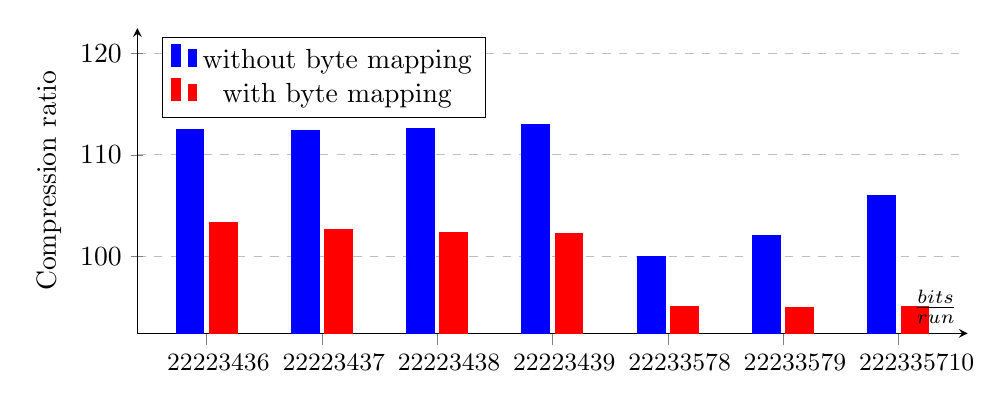
\begin{tikzpicture}
\begin{axis}[
width=\textwidth,
height=0.45\textwidth,
axis x line=center,
axis y line=left,
xlabel={$\frac{bits}{run}$},
ylabel={Compression ratio},
symbolic x coords={22223436,22223437,22223438,22223439,22233578,22233579,222335710},
x tick label style={font=\small,text width=1cm,align=center},
enlargelimits=true,
ymax=120,
legend pos=north west,
ymajorgrids=true,
grid style=dashed,
ybar]
\addplot[color=blue,fill]
	coordinates {
		(22223436,112.55)(22223437,112.4)(22223438,112.6)(22223439,113)(22233578,100)(22233579,102)(222335710,106)
	};
\addplot[color=red,fill]
coordinates {
	(22223436,103.3)(22223437,102.6)(22223438,102.3)(22223439,102.25)(22233578,95)(22233579,94.9)(222335710,95)
};
	\legend{without byte mapping,with byte mapping}
\end{axis}
\end{tikzpicture}
%}
%\end{scaletikzpicturetowidth}
\caption{Byte mapping and varying maximum run lengths}
\label{fig:2:Byte mapping and varying maximum run lengths}
\end{figure}

\par{
Using this combined approach the first time a real compression was achieved for the corpus instead of just one very specific file. The combination of 2 bits for the most insignificant bits, 3 for the fourth and fifth most insignificant bit 5 for the sixths most one, 7 bits for the second most significant bit and 9 bits for the most significant one yielded the overall best results with 94.9\% of its original size and 7.59 $\frac{bits}{symbol}$ as shown in Figure \ref{fig:2:Byte mapping and varying maximum run lengths}. Some files got a little smaller while other files still expanded which is only somewhat of an enhancement over regular RLE which performs really well on specific files. But on this corpus a slight reduction in size was achieved using preprocessing and a modified RLE.
\begin{table}[h]
	\centering
	\begin{tabular}{r|r|r|r|r}	
		file & size original & size encoded & ratio in \% & $\frac{bits}{symbol}$\\
		\hline
bib & 111261 & 111579 & 100.29 & 8.02 \\
book1 & 768771 & 669578 & 87.10 & 6.97 \\
book2 & 610856 & 551757 & 90.33 & 7.23 \\
geo & 102400 & 144974 & 141.58 & 11.33 \\
news & 377109 & 363010 & 96.26 & 7.70 \\
obj1 & 21504 & 30166 & 140.28 & 11.22 \\
obj2 & 246814 & 340165 & 137.82 & 11.03 \\
paper1 & 53161 & 50074 & 94.19 & 7.54 \\
paper2 & 82199 & 71747 & 87.28 & 6.98 \\
pic & 513216 & 408136 & 79.53 & 6.36 \\
progc & 39611 & 38490 & 97.17 & 7.77 \\
progl & 71646 & 63765 & 89.00 & 7.12 \\
progp & 49379 & 46093 & 93.35 & 7.47 \\
trans & 93695 & 94729 & 101.10 & 8.09 \\
		\hline
		all files & 3145718 & 2988359 & 94.99 & 7.59
	\end{tabular}
	\caption{Calgary Corpus encoded with vertical reading, byte remapping, using bits per run (2, 2, 3, 3, 3, 4, 5, 8)}
\label{tab:t43 Calgary Corpus encoded with vertical reading, byte remapping and varying bits per run}
\end{table}
}

\subsection{Burrows-Wheeler-Transformation Appliance}
\par{
Another possible preprocessing step which promised an improvement is the mentioned Burrows-Wheeler-Transformation from Section \ref{ch:Principles of compression:sec:Other:subSec:bwt}, initially applied to regular binary and byte wise RLE. By mistake a very simple transformation implementation was chosen, working by adding additional start and stop symbols to the input string (0x02 as STX, start of text and 0x03 as ETX, end of text). Some basic testing and playing around worked great but later on it revealed some major issues. For example the Calgary Corpus consists of more than textual data, in fact the files geo, obj1, obj2 and pic contain of some binary data of include the symbols STX or ETX so we wont be able to apply the transformation to these. Another shortcoming was the very poor time complexity of almost $O (n^2)$ because under the hood, it uses a dual pivot Quick-sort algorithm from the JDK 11, which is typically faster than traditional one pivot Quick-sort. This algorithm offers $\Theta (n \: log(n))$ average time complexity but in the worst case, its time complexity is cubic. This problem was partially solved by reading the input data in parts and performing the transformation on each part, result in a much smaller length $n$ and thus better run time at the expense of a slightly worse transformation result. As all chunks are individual transformations, they can also be computed in parallel without much effort.

\begin{table}[H]
	\centering
	\begin{tabular}{r|r|r}	
		bits per rle number & ratio in \% & bits per symbol in $\frac{bits}{symbol}$\\
		\hline
		3 & 95.41 & 7.63\\
		2 & 91.39 & 7.31 \\
	\end{tabular}
	\caption{Initial BWT implementation on byte wise RLE}
	\label{tab:t11 Simple Burrows Wheeler Transformation on byte wise RLE}
\end{table}
}
\par{
While it was only applicable to textual data and very slow, even when divided into smaller parts and computed in parallel, it improved the overall results of byte wise RLE by 16\% to a compression ratio of slightly over 7 $\frac{bits}{symbol}$ as table \ref{tab:t11 Simple Burrows Wheeler Transformation on byte wise RLE} depicts, which seemed like a good start. Regular binary RLE did not really benefit from this transformation as expected but on vertical interpretation, consecutive characters result in successive bits on every significance. Still this implementation had to be dropped and switched against one that could handle arbitrary input to be able to transform all files. This time all files could be processed and the resulting compression with byte wise RLE improved further as shown in table \ref{tab:t12 Burrows Wheeler Transformation on byte wise RLE}.

\begin{table}[H]
	\centering
	\begin{tabular}{r|r|r}	
		bits per rle number & ratio in \% & bits per symbol in $\frac{bits}{symbol}$\\
		\hline
		3 & 91.62 & 7.33\\
		2 & 89.46 & 7.15
	\end{tabular}
	\caption{Burrows Wheeler Transformation on byte wise RLE}
	\label{tab:t12 Burrows Wheeler Transformation on byte wise RLE}
\end{table}
}

\par{
In Section \ref{ch:Principles of compression:sec:Other} the Burrows-Wheeler-Transformation inversion was performed using a Matrix M containing all cyclic rotations of the input word, sorted in lexicographic order. However this is has a bad complexity and the inverting process does not even has access to this Matrix M.\\
}

\par{
In general a Burrows-Wheeler-Transformation should also increase the runs in the implementation of Section \ref{ch:Analysis:sec:Improvements by Preprocessing:subSec:vertReading} and \ref{ch:Analysis:sec:Improvements by Preprocessing:subSec:byteRemapping} so those preprocessing steps were also applied in combination. To do so, it was first swapped against an sufficient implementation provided by a paper from m. Burrows and D. J. Wheeler \cite{Burrows94} from 1994. Their method is also the one described in Section \ref{ch:Analysis:sec:Improvements by Preprocessing:subSec:bwt} and could handle arbitrary input but it also had some downsides like the additional index $I$ of the transformation, which had to be persisted as well. The major downside of this implementation although was the rather slow. To overcome this issue and the saving of additional indices, the implementation used had to be swapped once more against one that was first described by \cite{Burrows-linear-time} in 2009 which claimed to perform in linear time complexity.
}
\par{
In form of the C library \href{https://code.google.com/archive/p/libdivsufsort}{libdivsufsort} a working implementation of BWTS was found, the bijective Burrows-Wheeler-Scott-Transformation described in \cite{DBLP:journals/corr/abs-1201-3077}. This kind of Burrows-Wheeler-Transformation does not require additional information, no start and stop symbols neither and index of its original position. Briefly, it does not construct a matrix of all cyclic rotations, instead it is computed with a suffix array sorted with DivSufSort\cite{DBLP:journals/corr/abs-1710-01896} which is the fastest currently known method of constructing the transformation. To use it properly the code was ported to Kotlin but there are also ports of this library in Java and Go available which are recommended because the original code is neither documented nor readable and the functionality can easily be used via a dependency.
}
\par{
The simple binary RLE did not really benefit from this transformation which has to be expected, because it generates repetitions of bytes, but if a byte needs many short runs it will still expand in size because the average runs are not that much influenced. For example just the letter e needs 6 different runs, no matter on which position or surrounded by what letters. The byte wise implementation on the other hand did very strongly benefit from this transformation, it will always create longer runs of bytes. Swapping the implementation of the Burrows-Wheeler-Transformation resulted in way better results, the simple byte wise RLE archives compression ratios around 59 \% of its original size while using 4 bits per run, see table \ref{tab:t13 Modified Burrows Wheeler Transformation on byte wise RLE}. This was mainly because of the longer repetitions possible after the transformation was performed on the whole input instead of small chunks. This drastic increase was still a little astonishing but obviously average runs of characters increased so much, that 4 bits per run achieved the maximum result. Another reason for this vast improvement compared to the old implementations is the lack of additional information needed to store because we do no longer need to store the transformation index of every chunk or additional characters.
	\begin{table}[h]
		\centering
		\begin{tabular}{r|r|r}	
			bits per rle number & ratio in \% & bits per symbol in $\frac{bits}{symbol}$\\
			\hline
			8 & 74.42 & 5.95\\
			7 & 69.90 & 5.59\\
			6 & 65.58 & 5.24\\
			5 & 61.71 & 4.93\\
			4 & 58.98 & 4.71\\
			3 & 59.18 & 4.73\\
			2 & 67.69 & 5.41
		\end{tabular}
		\caption{Modified Burrows Wheeler Transformation on byte wise RLE}
		\label{tab:t13 Modified Burrows Wheeler Transformation on byte wise RLE}
	\end{table}
}
\par{
Working on the whole input data and no longer on small chunks, this BWTS generates extreme long runs of identical byte values, which in turn enhances the performance of the byte wise RLE vastly. If we take a closer look we can see in table \ref{tab:t14:Calgary Corpus encoded with byte wise RLE after a Burrows-Wheeler-Transformation} that all files have a compression ratio below 100 while the total size is nearly reduced to half. The file \textit{geo} is still close to uncompressed but half of the files only need less than 5 $\frac{bits}{symbol}$. The file \textit{pic} is still the best compressible with only 2.12 $\frac{bits}{symbol}$.
\begin{table}[H]
	\centering
	\begin{tabular}{r|r|r|r|r}	
		file & size original & size encoded & ratio in \% & $\frac{bits}{symbol}$\\
		\hline
bib & 111261 & 59285 & 53.28 & 4.26 \\
book1 & 768771 & 590879 & 76.86 & 6.15 \\
book2 & 610856 & 374742 & 61.35 & 4.91 \\
geo & 102400 & 101192 & 98.82 & 7.91 \\
news & 377109 & 246047 & 65.25 & 5.22 \\
obj1 & 21504 & 16467 & 76.58 & 6.13 \\
obj2 & 246814 & 126626 & 51.30 & 4.10 \\
paper1 & 53161 & 34130 & 64.20 & 5.14 \\
paper2 & 82199 & 56507 & 68.74 & 5.50 \\
pic & 513216 & 136074 & 26.51 & 2.12 \\
progc & 39611 & 24312 & 61.38 & 4.91 \\
progl & 71646 & 31466 & 43.92 & 3.51 \\
progp & 49379 & 20862 & 42.25 & 3.38 \\
trans & 93695 & 32835 & 35.04 & 2.80 \\
\hline
all files & 3145718 & 1855520 & 58.98 & 4.71
	\end{tabular}
	\caption{Calgary Corpus encoded with byte wise RLE after a Burrows-Wheeler-Transformation}
	\label{tab:t14:Calgary Corpus encoded with byte wise RLE after a Burrows-Wheeler-Transformation}
\end{table}
}
\par{
There should still room for some optimizations because as seen in Section \ref{ch:Conceptual Design:sec:var lengths}, the remapping of the input resulted in longer runs on the higher order bits and the vertical interpretation made it possible to encode different sections with different maximum run lengths. It was expected that applying the Burrows-Wheeler-Transformation to the vertical encoding variant should improve its efficiency as much as the byte wise RLE did benefit, which turned out to be wrong. The vertical interpretation did indeed perform at its best when applying the BWTS and the mapping but it did not outperform the combination of BWTS and byte wise RLE which is kind of expected because the transformation creates repetitions on byte level.

\begin{figure}[h]
	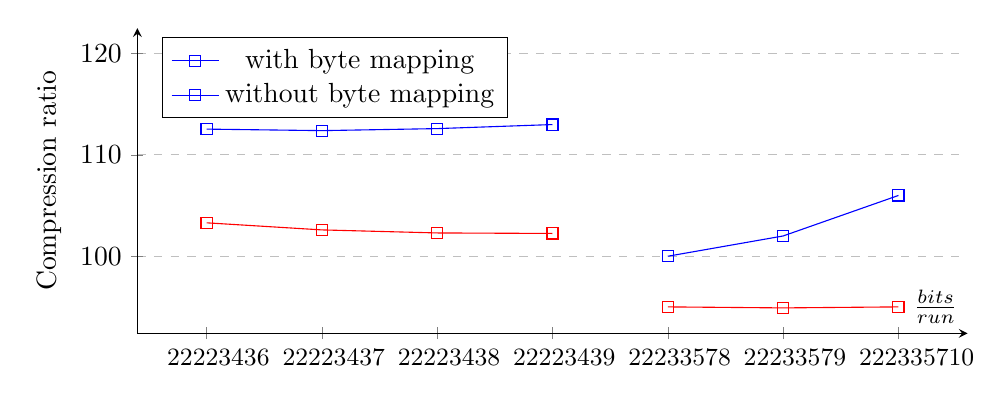
\begin{tikzpicture}
	\begin{axis}[
	width=\textwidth,
	height=0.45\textwidth,
	axis x line=center,
	axis y line=left,
	xlabel={$\frac{bits}{run}$},
	ylabel={Compression ratio},
	symbolic x coords={22223436,22223437,22223438,22223439,22233578,22233579,222335710},
	x tick label style={font=\small,text width=1cm,align=center},
	enlargelimits=true,
	ymax=120,
	legend pos=north west,
	ymajorgrids=true,
	grid style=dashed
	]
	\addplot[color=blue,mark=square]
	coordinates {
		(22223436,112.55)(22223437,112.4)(22223438,112.6)(22223439,113)
	};
	\addplot[color=blue,mark=square]
	coordinates {
		(22233578,100)(22233579,102)(222335710,106)
	};
	\addplot[color=red,mark=square]
	coordinates {
		(22223436,103.3)(22223437,102.6)(22223438,102.3)(22223439,102.25)
	};
	\addplot[color=red,mark=square]
	coordinates {
	(22233578,95)(22233579,94.9)(222335710,95)
	};
	\legend{with byte mapping, without byte mapping}
	\end{axis}
	\end{tikzpicture}
	%}
	%\end{scaletikzpicturetowidth}
	\caption{Byte mapping and varying maximum run lengths}
	\label{fig:3:Different run lengths with and without transformations}
\end{figure}

\par{
	TODO: explain
\begin{table}[h]
	\centering
	\begin{tabular}{r|r|r|r|r}	
		file & size original & size encoded & ratio in \% & $\frac{bits}{symbol}$\\
		\hline
		bib & 111261 & 73843 & 66.37 & 5.31 \\
		book1 & 768771 & 570348 & 74.19 & 5.94 \\
		book2 & 610856 & 409639 & 67.06 & 5.36 \\
		geo & 102400 & 145950 & 142.53 & 11.40 \\
		news & 377109 & 275396 & 73.03 & 5.84 \\
		obj1 & 21504 & 27023 & 125.66 & 10.05 \\
		obj2 & 246814 & 213392 & 86.46 & 6.92 \\
		paper1 & 53161 & 37344 & 70.25 & 5.62 \\
		paper2 & 82199 & 56490 & 68.72 & 5.50 \\
		pic & 513216 & 227914 & 44.41 & 3.55 \\
		progc & 39611 & 28275 & 71.38 & 5.71 \\
		progl & 71646 & 38144 & 53.24 & 4.26 \\
		progp & 49379 & 27029 & 54.74 & 4.38 \\
		trans & 93695 & 49314 & 52.63 & 4.21 \\
		\hline
		all files & 3145718 & 2184197 & 69.43 & 5.55
	\end{tabular}
	\caption{Calgary Corpus encoded, all preprocessing steps, using bits per run: 4, 4,4, 4, 5, 7, 8, 10}
	\label{tab:t5:Calgary Corpus encoded, all preprocessing steps, using bits per run: 4, 4,4, 4, 5, 7, 8, 10}
\end{table}

\par{
One last option was the encoding of the lowest significant bits with another, more suited scheme like Huffman encoding was tried out but with rather poor results. It was found that encoding the last or the last few rows seen in \ref{ch:Analysis:sec:Improvements by Preprocessing:subSec:vertReading} with did not improve overall results and it was therefore discarded. This might be related to the high improvement in RLE after a Burrows-Wheeler-Transformation and other factors like additional overhead because the mapping of the Huffman encoding has to be persisted with the encoded data. But the idea of combing the RLE methods with Huffman encoding still stuck around and was picked up again later on in a modified way in Section \ref{ch:Conceptual Design:sec:Postprocessing}. No further attempts to add or improve preprocessing steps of this kind were made, instead the results were analyzed and compared with other results in section \ref{ch:Evaluation}.
}
%% ==============================
\subsection{Huffman encoding of the RLE runs}
%% ==============================
\label{ch:Conceptual Design:sec:Postprocessing}
\par{
Another step worth mentioning was the encoding using Huffman codes after the Run length encoding was performed, similar to the Fax Transmission Standard mentioned in section \ref{ch:Principles of compression:sec:Run Length Encoding:subSec:History}, but i a dynamic way instead of predefined static codes. This idea was also used by Burrows and Wheeler in their paper \cite{Burrows94} but instead of RLE they combined a Move to Front Coder with their transformation and then encoded the result using Huffman codes. This way it would be possible to encode more frequent results of the Move to Front Encoder or the Run Length Encoder could be encoded into shorter codes and thus save even more space. This step is not really considered preprocessing anymore but could improve the compression furthermore, however the benefit of Huffman encoding is the possibility to output codes of varying length as described in section \ref{ch:Principles of compression:sec:Huffman Coding}. Combining the binary or vertical encoded RLE with a Huffman encoder would be a huge benefit, because as of now the algorithm needs to output a number of bits for each number to encode. Combined, the more frequent short runs of 1 or 2 can be encoded into shorter Huffman codes which should increase the overall compression algorithm. In general it was assumed that there was no longer a benefit in using different maximum run lengths on bits of different significance, because a run of length 1 is going to be encoded with a Huffman code, not with the fixed amount of bits. To reverse the Huffman encoding, the Huffman tree has to be persisted into the file as well.
}
%% ==============================
\section{Implementation}
%% ==============================
\label{ch:Conceptual Design:sec:Implementation Decisions}

The algorithms described have all been implemented using Kotlin, because it can be compiled for the Java Virtual Machine as well as native, so it seemed like a good balance between native speed and higher language conciseness and fault-tolerance. Also there were some library available for Byte- and Bit-Operations on streams which proved to be quite useful.

%% ==============================
\subsection{Implementation Detail}
%% ==============================
\label{ch:Conceptual Design:sec:Implementation Detail}
- detailed information about specific modules and classes\\
\ldots

\subsection{Burrows Wheeler Transformation}
- TBD\\
\subsection{Byte Remapping}
- show use case \\

%% ==============================
\section{Implementation Evaluation}
%% ==============================
\label{ch:Conceptual Design:sec:Implementation Evaluation}
- evaluation of implementation choices made


%% ==============================
\section{Summary}
%% ==============================
\label{ch:Conceptual Design:sec:Summary}

Am Ende sollten ggf. die wichtigsten Ergebnisse nochmal in \emph{einem}
kurzen Absatz zusammengefasst werden.

%%% Local Variables: 
%%% mode: latex
%%% TeX-master: "thesis"
%%% End: 
